% ============================================================================
% Saturable Vacuum Electrodynamics: A Tree-Level Vacuum Birefringence
% Prediction for BIREF@HIBEF
%
% Standalone, self-contained, pre-registered prediction Letter.
% Every quantitative claim traces to a single constitutive postulate (Sec. II).
% Working model name flagged for author decision (see PR).
% Build:  pdflatex main && bibtex main && pdflatex main && pdflatex main
% ============================================================================
\documentclass[aps,prd,twocolumn,superscriptaddress,nofootinbib,longbibliography]{revtex4-2}

\usepackage{amsmath,amssymb}
\usepackage{graphicx}
\usepackage{booktabs}
\usepackage{siunitx}
\usepackage[colorlinks=true,allcolors=blue]{hyperref}

\sisetup{range-phrase=--,range-units=single}

\newcommand{\Ec}{E_{\mathrm{c}}}
\newcommand{\Ecrit}{E_{\mathrm{crit}}}
\newcommand{\dnbir}{\delta n_{\mathrm{bir}}}
\newcommand{\Pflip}{P_{\mathrm{flip}}}

\begin{document}

\title{Saturable Vacuum Electrodynamics: a tree-level vacuum-birefringence
prediction for a pump--probe X-ray polarimeter}

\author{G.~Lindblom}
\email{grant6t@gmail.com}
\affiliation{Independent researcher}

\date{\today}

\begin{abstract}
We register, before any pump-on data exists, a falsifiable prediction for the
combined optical-pump / X-ray-probe polarimeter geometry of the BIREF@HIBEF
proposal. The prediction follows from a single constitutive postulate: the
vacuum permittivity saturates as $\varepsilon_{\mathrm{eff}}=\varepsilon_0\,
S(E)$ with the quarter-arc kernel $S=\sqrt{1-(E/\Ec)^2}$ and one field scale
$\Ec\simeq\SI{1.13e17}{\volt\per\meter}$. Under a linearly polarized pump this
yields a \emph{tree-level}, $E^2$-leading birefringence $\dnbir=n_\parallel-
n_\perp\simeq-\tfrac12(E/\Ec)^2$ whose differential coefficient exceeds the
one-loop QED (Euler--Heisenberg) prediction by the field-independent factor
$\delta n_{\mathrm{AVE}}/\delta n_{\mathrm{QED}}=7.5/\alpha^3\simeq
\num{1.93e7}$. At the demonstrated ReLaX pump intensity
($\SI{e21}{\watt\per\centi\meter\squared}$) the model predicts a
polarization-flip probability $\Pflip\simeq\numrange{4e-3}{9e-3}$, roughly
seven orders of magnitude above the demonstrated X-ray-polarimeter purity floor
($\num{2.4e-10}$). The model's magnetic response keys on circulation rather
than static flux, so it predicts \emph{zero} static-magnetic-field
birefringence; existing PVLAS/BMV magnetic nulls are therefore consistent by
construction, and the E-route configuration is the decisive one. We state the
kill criterion explicitly: a pump-on polarimetric null at or below the QED
co-prediction, above the demonstrated purity floor and at
$\gtrsim\SI{e18}{\watt\per\centi\meter\squared}$, falsifies the model's
electric sector. Because the signal sits $\sim\!10^7$ above the demonstrated
floor at already-demonstrated parameters, even commissioning-grade data
adjudicates it. We report the coefficient honestly: the kernel \emph{form} and
the resulting coefficient \emph{structure} are the model's content, whereas the
absolute scale $\Ec$ is calibrated from the same measured constants
($\alpha$, $m_e$) that fix the QED prediction.
\end{abstract}

\maketitle

% ============================================================================
\section{Introduction}
% ============================================================================

Quantum electrodynamics predicts that the vacuum, polarized by an intense
electromagnetic field, becomes weakly birefringent~\cite{HeisenbergEuler1936,
Schwinger1951}. The effect is an $\alpha^2$-suppressed one-loop response: for a
probe crossing a field of strength $E$ the two eigenmodes acquire an index
difference $\delta n_{\mathrm{QED}}\sim\alpha^2(E/\Ecrit)^2$, with
$\Ecrit=m_e^2c^3/(e\hbar)\simeq\SI{1.3e18}{\volt\per\meter}$ the Schwinger
field. The predicted signal is minute and has never been measured directly. The
BIREF@HIBEF proposal~\cite{BirefHibefLoI2025} targets it with a pump--probe
geometry at the European XFEL: a petawatt-class optical laser (ReLaX) supplies
the strong field and a polarized X-ray pulse probes the induced birefringence
through a high-purity crossed polarimeter.

This Letter registers a competing, tree-level prediction for the \emph{same}
observable in the \emph{same} apparatus. It rests on one constitutive
hypothesis for the vacuum's dielectric response --- that the permittivity
\emph{saturates} with field strength through a specific quarter-arc kernel ---
which we treat here as a self-contained model of nonlinear electrodynamics,
neutral to any wider interpretation. We call it saturable vacuum
electrodynamics (SVE). The model makes a numerically definite, pre-committed
prediction that differs from QED by a fixed, field-independent factor, and it
carries a distinctive signature --- electric-field-active but
static-magnetic-field-transparent --- that separates it from both QED and the
Born--Infeld class of nonlinear electrodynamics~\cite{BornInfeld1934}, in which
electric and magnetic responses are symmetric.

Our aim is a clean falsifier, not a defense. We therefore (i) state the model
as a two-parameter constitutive law with its one calibrated scale ledgered
plainly; (ii) compute the prediction and the QED co-prediction through an
identical readout chain; (iii) show that no published experiment has yet
combined a strong optical pump, a polarized X-ray probe, and a polarization-flip
analysis, so this is a forward prediction rather than a retrodiction; and
(iv) commit, before data, to the measurement outcome that would kill the model.

% ============================================================================
\section{The constitutive model}
\label{sec:model}
% ============================================================================

\subsection{The saturable permittivity}

We postulate that the vacuum responds to an applied electric field as a
dielectric whose permittivity \emph{saturates} rather than remaining constant.
Concretely, with $\varepsilon_0$ the low-field vacuum permittivity, we take the
effective permittivity along the field to be
%
\begin{equation}
  \varepsilon_{\mathrm{eff}}(E)=\varepsilon_0\,S(E),\qquad
  S(E)=\sqrt{1-\left(\frac{E}{\Ec}\right)^2},
  \label{eq:kernel}
\end{equation}
%
a single quarter-arc kernel controlled by one field scale $\Ec$. The functional
form is the defining hypothesis: $S$ is unity at low field, softens as $E$
grows, and reaches zero at $E=\Ec$, where the medium ceases to support
propagation. Equation~\eqref{eq:kernel} is the only nonlinearity in the model;
everything below is its consequence.

For a linearly polarized pump field $\mathbf E_0$ the response becomes uniaxial,
with optic axis along $\hat{\mathbf E}_0$. Writing $A\equiv E/\Ec$, the
probe-response tensor is the exact differential of the scalar kernel,
$\varepsilon_{ij}=\varepsilon\,\delta_{ij}+2\varepsilon'E_{0i}E_{0j}$ with
$\varepsilon'=\mathrm d\varepsilon/\mathrm d(E^2)$. The two refractive
eigen-indices for a probe are
%
\begin{equation}
  n_\perp=(1-A^2)^{1/4},\qquad
  n_\parallel=\sqrt{\frac{1-2A^2}{\sqrt{1-A^2}}},
  \label{eq:eigenindices}
\end{equation}
%
and the birefringence a polarimeter measures is their difference,
%
\begin{equation}
  \boxed{\;\dnbir=n_\parallel-n_\perp\;\simeq\;-\tfrac12 A^2
  =-\tfrac12\left(\frac{E}{\Ec}\right)^2\;}
  \label{eq:dnbir}
\end{equation}
%
to leading order in $A$. This is negative, $E^2$-leading, and $O(1)$ against the
saturation scale $\Ec$ --- it is not loop-suppressed. It vanishes at low field
($A\to0$), recovering an unbirefringent tree-level vacuum exactly as QED does at
tree level; the distinction from QED is one of \emph{coefficient}, at the same
leading power (Sec.~\ref{sec:prediction}).

\subsection{The one calibrated scale}

The kernel~\eqref{eq:kernel} has one dimensionful parameter, the saturation
field $\Ec$. We fix it as
%
\begin{equation}
  \Ec=\sqrt{\alpha}\,\Ecrit,\qquad
  \Ecrit=\frac{m_e^2c^3}{e\hbar},
  \label{eq:Ec}
\end{equation}
%
which evaluates to $\Ec\simeq\SI{1.13e17}{\volt\per\meter}$ using the fine
structure constant $\alpha$ and the electron mass $m_e$. Equation~\eqref{eq:Ec}
places the saturation field a factor $\sqrt{\alpha}$ below the QED Schwinger
field $\Ecrit\simeq\SI{1.3e18}{\volt\per\meter}$, and it is the origin of the
field-independent ratio to QED derived below, through the exact identity
%
\begin{equation}
  \left(\frac{\Ecrit}{\Ec}\right)^2=\frac1\alpha .
  \label{eq:identity}
\end{equation}

\paragraph*{Honesty ledger.}
We separate what the model supplies from what it imports, and we hold it to the
same standard as QED.
\emph{(i) The kernel form is the model's content.} That the vacuum saturates at
all --- possessing a tree-level, $O(1)$, birefringence-bearing structure --- is
the substantive, potentially wrong hypothesis. The QED vacuum has no such
tree-level structure; its birefringence is an $\alpha^2$-loop effect. The
existence and functional form of Eq.~\eqref{eq:kernel} is therefore the
distinguishing physics.
\emph{(ii) The coefficient structure is the model's content.} The factors of
$\tfrac12$ in Eq.~\eqref{eq:dnbir} and $\sqrt\alpha$ in Eq.~\eqref{eq:Ec}, and
hence the $\alpha^{-3}$ scaling of the ratio to QED, follow from the form once
$\Ec$ is fixed.
\emph{(iii) The absolute scale is calibrated, not derived.} The number
$\Ec\simeq\SI{1.13e17}{\volt\per\meter}$ is set through Eq.~\eqref{eq:Ec} from
the \emph{same} measured constants ($\alpha$, $m_e$) that every treatment of
this problem imports; the model does not predict $\alpha$. The resulting
magnitude of the ratio to QED, $7.5/\alpha^3$, is thus rooted in $\alpha$ in
exactly the way QED's own coefficient $a_{\mathrm{EH}}\,\alpha^2$ is: neither
framework derives $\alpha$. We therefore do not present the numerical magnitude
as the discriminating claim. The discriminating claim is the \emph{existence of
an $O(1)$ tree-level differential coefficient} where QED has only an
$\alpha^2$-loop one --- and this is what the experiment tests.

\subsection{The magnetic sector: static-flux transparency}

The constitutive postulate is completed by a statement about the magnetic
response, which is \emph{not} symmetric with the electric one. In this model the
magnetic response of the vacuum keys on the \emph{circulation} of the field ---
the time-varying, curl-carrying part --- rather than on static flux. A purely
static magnetic field ($\partial\mathbf B/\partial t=0$) does not load the
magnetic response: the corresponding saturation factor stays at unity and the
magnetic-route birefringence is
%
\begin{equation}
  \delta n_\mu=0\qquad(\text{static }\mathbf B,\ \text{exactly}).
  \label{eq:staticB}
\end{equation}
%
This is a hard, parameter-free side-prediction: the model forbids
static-magnetic-field vacuum birefringence at any field strength. It is the
feature that most sharply separates the model from QED and from Born--Infeld-type
electrodynamics, both of which predict a nonzero static-$\mathbf B$
birefringence. A propagating field --- such as the ReLaX optical pump, for which
$\mathbf E$ and $\mathbf B$ co-move with $B=E/c$ and $\partial\mathbf
B/\partial t\ne0$ --- \emph{does} load the response; the electric-route result
of Eq.~\eqref{eq:dnbir} already captures the full birefringence of such a wave.
The consequences of Eq.~\eqref{eq:staticB} for existing null experiments are
taken up in Sec.~\ref{sec:signature}.

% ============================================================================
\section{The prediction}
\label{sec:prediction}
% ============================================================================

\subsection{The matched differential and the readout chain}

A birefringence polarimeter measures the \emph{difference} $n_\parallel-n_\perp$
between the two eigenmodes; the common-mode index shift shared by both modes is
rejected by the instrument. The falsifier observable is therefore the
differential $\dnbir$ of Eq.~\eqref{eq:dnbir}, and any comparison with QED must
be made differential-against-differential. The QED (Euler--Heisenberg)
birefringence, differenced the same way, is
%
\begin{equation}
  \delta n_{\mathrm{QED}}=\frac{3}{45}\,\alpha^2
  \left(\frac{E}{\Ecrit}\right)^2,
  \label{eq:dnqed}
\end{equation}
%
the parallel ($7/45$) and perpendicular ($4/45$) one-loop eigen-coefficients
differenced. Both Eq.~\eqref{eq:dnbir} and Eq.~\eqref{eq:dnqed} are
$E^2$-leading: an $E^2$ slope alone does \emph{not} discriminate the two. The
discriminator is the coefficient.

For a single-pass geometry (no cavity build-up), an index difference $\dnbir$
over an interaction length $z$ imprints a retardance
$\Delta\varphi=(2\pi/\lambda)|\dnbir|\,z$ on a probe of wavelength $\lambda$,
rotating a fraction
%
\begin{equation}
  \Pflip=\sin^2\!\left(\frac{\Delta\varphi}{2}\right)
  \label{eq:flip}
\end{equation}
%
of the probe intensity into the crossed polarimeter channel. This bounded form
reduces to the perturbative $(\Delta\varphi/2)^2$ when $\Delta\varphi\ll1$. We
compute both the model and the QED co-prediction through this \emph{identical}
chain, changing only $\dnbir$, so the comparison is like-for-like and free of a
strawman baseline.

\subsection{The field-independent ratio}

Because both responses are $E^2$-leading, their ratio is independent of field
strength. Using Eqs.~\eqref{eq:dnbir}, \eqref{eq:dnqed}, and the
identity~\eqref{eq:identity},
%
\begin{equation}
  \frac{\delta n_{\mathrm{AVE}}}{\delta n_{\mathrm{QED}}}
  =\frac{1/2}{(3/45)\,\alpha^2}\left(\frac{\Ecrit}{\Ec}\right)^2
  =\frac{45/6}{\alpha^3}=\frac{7.5}{\alpha^3}\simeq\num{1.93e7}.
  \label{eq:ratio}
\end{equation}
%
The model predicts a differential coefficient nearly eight orders of magnitude
larger than QED's, at every field. As stressed in the honesty ledger, the
\emph{value} $7.5/\alpha^3$ is $\alpha$-rooted --- as is QED's own coefficient
--- and is not itself the claim; the claim is the existence of an $O(1)$
tree-level differential where QED has only a loop.

\subsection{Per-scenario predictions}

Table~\ref{tab:scenarios} freezes the prediction for the scenarios of the
BIREF@HIBEF proposal~\cite{BirefHibefLoI2025}: the probe photon energies of the
conventional, dark-field, and high-energy configurations, at the demonstrated
ReLaX pump intensity and at the higher design intensities, through the
single-pass chain of Eqs.~\eqref{eq:flip} with $z=\SI{10}{\micro\meter}$. At the
\emph{demonstrated} pump ($\SI{e21}{\watt\per\centi\meter\squared}$,
$E\simeq\SI{8.7e13}{\volt\per\meter}$, $A^2\simeq\num{5.9e-7}$) the retardance is
small ($\Delta\varphi/2\lesssim0.1$) and the flip probability is a well-behaved
$\Pflip\simeq\numrange{4e-3}{9e-3}$ across the three probe energies --- no
non-perturbative regime is invoked. The QED co-prediction at the same parameters
is $\sim\!\num{e-17}$. The two hypotheses are separated by roughly fourteen
orders of magnitude in flip probability.

\begin{table*}[t]
  \centering
  \caption{Frozen per-scenario predictions for the BIREF@HIBEF probe energies,
  computed through the single-pass readout chain [Eqs.~\eqref{eq:dnbir},
  \eqref{eq:dnqed}, \eqref{eq:flip}] at $z=\SI{10}{\micro\meter}$. The three
  demonstrated-pump rows are the bankable prediction. The two design rows are
  shown for context: the $\SI{e22}{\watt\per\centi\meter\squared}$ row is
  saturating (retardance $\Delta\varphi=\SI{1.47}{\radian}$, so the small-angle
  approximation no longer holds and the exact $\sin^2$ value is quoted), and the
  $\SI{e23}{\watt\per\centi\meter\squared}$ row (retardance
  $\Delta\varphi=\SI{14.7}{\radian}$, many-wrap) is a named validity limit of
  the single-pass mapping and is \emph{not} part of the registered prediction
  (Sec.~\ref{sec:falsify}).}
  \label{tab:scenarios}
  \begin{ruledtabular}
  \begin{tabular}{lccccccc}
    Scenario (probe) & Pump [\si{\watt\per\centi\meter\squared}] & $E$ [\si{\volt\per\meter}] & $A^2$ & $\Pflip$ (model) & $\Pflip$ (QED) & model/QED & regime \\
    \colrule
    Conventional (\SI{9835}{\electronvolt})   & \num{e21} (demonstrated) & \num{8.68e13} & \num{5.90e-7} & \num{5.39e-3} & \num{1.45e-17} & \num{3.72e14} & small-angle \\
    Dark-field (\SI{8766}{\electronvolt})     & \num{e21} (demonstrated) & \num{8.68e13} & \num{5.90e-7} & \num{4.28e-3} & \num{1.15e-17} & \num{3.72e14} & small-angle \\
    High-energy (\SI{12914}{\electronvolt})   & \num{e21} (demonstrated) & \num{8.68e13} & \num{5.90e-7} & \num{9.28e-3} & \num{2.50e-17} & \num{3.71e14} & small-angle \\
    \colrule
    Conventional (\SI{9835}{\electronvolt})   & \num{e22} (design) & \num{2.74e14} & \num{5.90e-6} & \num{4.49e-1} & \num{1.45e-15} & \num{3.10e14} & saturating \\
    Conventional (\SI{9835}{\electronvolt})   & \num{e23} (design) & \num{8.68e14} & \num{5.90e-5} & \num{7.65e-1} & \num{1.45e-13} & \num{5.28e12} & beyond validity \\
  \end{tabular}
  \end{ruledtabular}
\end{table*}

% ============================================================================
\section{The signature and prior nulls}
\label{sec:signature}
% ============================================================================

The model's identifying signature is that it is \emph{electric-route active but
static-magnetic-route transparent} [Eq.~\eqref{eq:staticB}]. This distinguishes
it from both of the standard alternatives. QED predicts a nonzero
static-$\mathbf B$ vacuum birefringence, and the entire PVLAS/BMV program was
built to detect exactly that; Born--Infeld-type nonlinear
electrodynamics~\cite{BornInfeld1934} likewise predicts symmetric electric and
magnetic responses. The present model predicts none in a static magnetic field.

A consequence is that the existing magnetic-route nulls are consistent with this
model \emph{by construction}, not by smallness of a coefficient. The PVLAS
experiment, in a 25-year effort, measured no vacuum magnetic birefringence at a
sensitivity approaching the QED prediction~\cite{Ejlli2020}. In this model that
null is required: $\delta n_\mu=0$ exactly for static $\mathbf B$. The
magnetic-route facilities therefore neither support nor test the present
prediction; they confirm the side-prediction of Eq.~\eqref{eq:staticB} and leave
the electric route open.

The electric route requires a strong \emph{propagating} field crossed by a
polarized probe --- precisely the XFEL-plus-optical-laser geometry. Theory for
the QED signal in this configuration is well
developed~\cite{Karbstein2015,BirefHibefLoI2025}; the same geometry is the
uniquely decisive test of the present model, because it is the one configuration
in which the model and QED both predict a nonzero, matched, differential signal
and differ only in coefficient.

% ============================================================================
\section{Falsifiability}
\label{sec:falsify}
% ============================================================================

We commit, before any pump-on data, to the following outcome as decisive.

\paragraph*{Kill criterion.}
A pump-on polarimetric run at
$\gtrsim\SI{e18}{\watt\per\centi\meter\squared}$, with a polarimeter operating
at or below the demonstrated purity floor, that measures a polarization-flip
probability at or below the QED co-prediction --- i.e.\ no signal of the
model's predicted size where the polarimeter can resolve it --- falsifies the
electric sector of this model. This is a QED-sized differential coefficient
where the model demands an $O(1)$ one, and we record it as a clean
falsification: the model's electric-route hypothesis is closed, with no rescue.
Conversely, a measured flip probability of the predicted size
($\numrange{4e-3}{9e-3}$ at the demonstrated pump, some seven orders of
magnitude above the floor) is inconsistent with QED at this observable.

\paragraph*{Why commissioning data suffices.}
The highest X-ray-polarimeter purity demonstrated to date is
$\num{2.4e-10}$~\cite{Marx2013}, measured with the pump off. At the demonstrated
ReLaX intensity the model predicts $\Pflip\simeq\numrange{4e-3}{9e-3}$
(Table~\ref{tab:scenarios}), which sits a factor $\sim\!\num{2e7}$ above that
floor. The prediction is thus not a precision measurement at the edge of
feasibility: it is a $\sim\!10^7$ effect at already-demonstrated parameters, so
even a commissioning-grade pump-on polarimetric measurement adjudicates it.
Figure~\ref{fig:exposure} places the prediction, the QED co-prediction, the
demonstrated floor, and the demonstrated pump on the exposure plane.

\paragraph*{This is a forward prediction.}
No published experiment has combined a strong optical pump, a polarized X-ray
probe, and a polarization-flip analysis at the required geometry. The reported
$\num{8e-11}$--$\num{2.4e-10}$ polarimeter purities were measured with the pump
off~\cite{Marx2013,BirefHibefLoI2025}; the March-2024 HIBEF beamtime was
X-ray-only, with the optical pump not fired~\cite{BirefHibefLoI2025}; the
all-optical and X-ray--X-ray light-by-light searches, the heavy-ion
measurements, and the PVLAS magnetic-route null~\cite{Ejlli2020} all lack the
combination of a polarized X-ray probe passing through a strong optical focus
with flip analysis. The exposure region that would bound the model's E-route
signal is therefore empty (Fig.~\ref{fig:exposure}), and the present table is a
pre-registration rather than a retrodiction.

\paragraph*{An honest exclusion.}
The highest design intensity of the proposal,
$\SI{e23}{\watt\per\centi\meter\squared}$, drives the single-pass retardance to
$\Delta\varphi\simeq\SI{14.7}{\radian}$ (Table~\ref{tab:scenarios}). In this
many-wrap regime the crossed-polarimeter flip fraction of Eq.~\eqref{eq:flip} is
a rapidly oscillating function whose single-pass interpretation is not credible.
We do \emph{not} register a prediction there; it is a named validity limit of
the readout mapping, not part of the falsifier. The registered prediction lives
entirely at the demonstrated-pump scenarios, where the small-angle mapping
holds.

\begin{figure}[t]
  \centering
  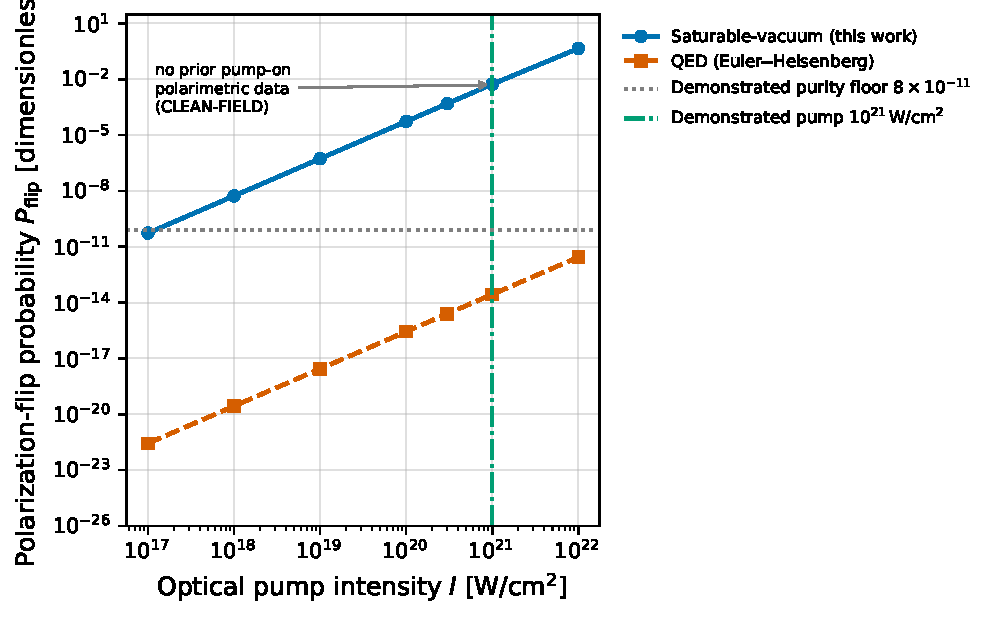
\includegraphics[width=\columnwidth]{figures/exposure_plane.pdf}
  \caption{The exposure plane. Predicted polarization-flip probability $\Pflip$
  versus optical-pump intensity for the saturable-vacuum model (blue,
  Eqs.~\eqref{eq:dnbir} and \eqref{eq:flip}) and for the QED Euler--Heisenberg
  co-prediction (orange), through the identical single-pass readout chain at
  probe energy \SI{9835}{\electronvolt}, $z=\SI{10}{\micro\meter}$. Both scale
  as intensity squared, so their ratio is field-independent. The demonstrated
  X-ray-polarimeter purity floor ($\num{8e-11}$, dotted) and the demonstrated
  ReLaX pump intensity ($\SI{e21}{\watt\per\centi\meter\squared}$, dash-dot) are
  marked. No prior experiment occupies the pump-on polarimetric exposure region,
  so the model's prediction there is unconstrained by existing data.}
  \label{fig:exposure}
\end{figure}

% ============================================================================
\section{Conclusion}
% ============================================================================

A single constitutive postulate --- a vacuum permittivity that saturates through
the quarter-arc kernel of Eq.~\eqref{eq:kernel}, with one calibrated field scale
--- yields a definite, pre-registered, tree-level birefringence prediction for
the pump--probe X-ray polarimeter geometry of BIREF@HIBEF. The prediction
exceeds the QED co-prediction by the field-independent factor $7.5/\alpha^3$,
sits $\sim\!10^7$ above the demonstrated polarimeter floor at already-demonstrated
pump parameters, and carries a hard side-prediction --- no static-magnetic-field
vacuum birefringence --- that renders the existing PVLAS/BMV nulls consistent by
construction and singles out the electric-route XFEL geometry as decisive. We
have stated the kill criterion in advance and ledgered the one imported scale
plainly. The measurement that decides the model is within reach of
commissioning-grade data at an already-operating facility.

\bibliographystyle{apsrev4-2}
\bibliography{refs}

\end{document}
